\newproblem{16a}
{
	Identify the slope and the y-intercept of the line graphed below.
	\begin{center}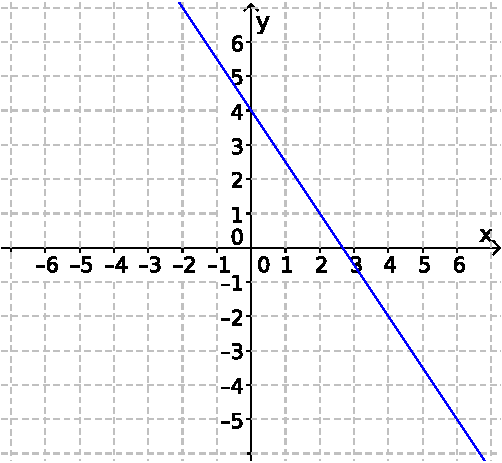
\includegraphics{fig095-11-a}\end{center}
}
{
	\begin{tabular}{l r}
	$m=-\frac{3}{2}$ or $-1.5$ & $3.5$ pts\\
	$b=4$ or $(0,4)$ & 3.5 pts
	\end{tabular}
}

\newproblem{16b}
{
	Identify the slope and the y-intercept of the line graphed below.
	\begin{center}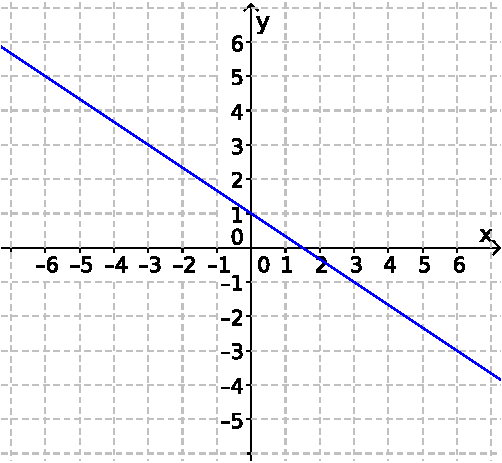
\includegraphics{fig095-11-b}\end{center}
}
{
	\begin{tabular}{l r}
	$m=-\frac{2}{3}$ or $-0.67$ & $3.5$ pts\\
	$b=1$ or $(0,1)$ & 3.5 pts
	\end{tabular}
}

\newproblem{16c}
{
	Identify the slope and the y-intercept of the line graphed below.
	\begin{center}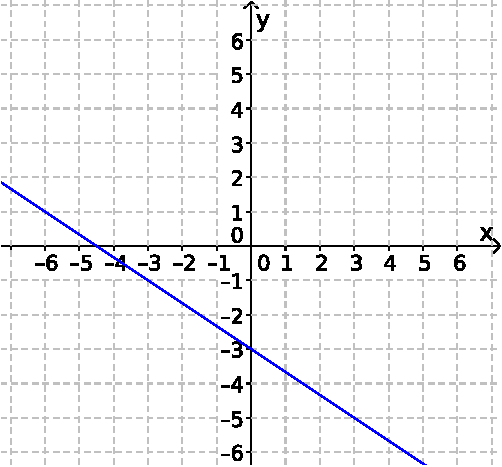
\includegraphics{fig095-11-c}\end{center}
}
{
	\begin{tabular}{l r}
	$m=-\frac{2}{3}$ or $-0.67$ & $3.5$ pts\\
	$b=-3$ or $(0,-3)$ & 3.5 pts
	\end{tabular}
}

\newproblem{16d}
{
	Identify the slope and the y-intercept of the line graphed below.
	\begin{center}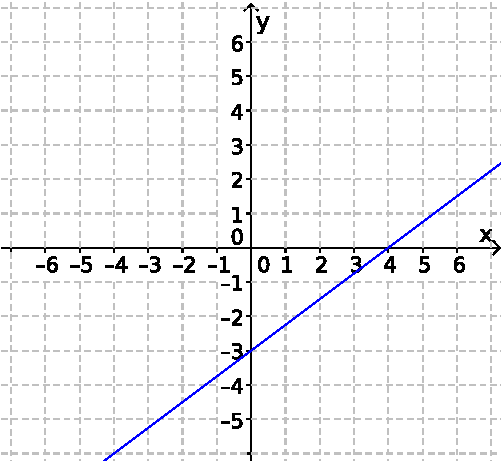
\includegraphics{fig095-11-d}\end{center}
}
{
	\begin{tabular}{l r}
	$m=\frac{3}{4}$ or $0.75$ & $3.5$ pts\\
	$b=-3$ or $(0,-3)$ & 3.5 pts
	\end{tabular}
}
